%%
%% prog-folien
%%
%% Slides for my Java programming tutorial using LaTeX beamer.
%%
%% Copyright (c) 2015-2016 YouniS Bensalah <younis.bensalah@gmail.com>
%%
%% This work is released to the public domain.
%% For the full copyright and license information, please view the LICENSE file.
%%

%% LaTeX-Beamer template for KIT design
%% by Erik Burger, Christian Hammer
%% title picture by Klaus Krogmann
%%
%% version 2.1
%%
%% mostly compatible to KIT corporate design v2.0
%% http://intranet.kit.edu/gestaltungsrichtlinien.php
%%
%% Problems, bugs and comments to
%% burger@kit.edu

\documentclass[18pt]{beamer}

%% SLIDE FORMAT

% use 'beamerthemekit' for standard 4:3 ratio
% for widescreen slides (16:9), use 'beamerthemekitwide'

\usepackage{templates/beamerthemekit}
% \usepackage{templates/beamerthemekitwide}

\usepackage[utf8]{inputenc}
\usepackage{hyperref}
\usepackage{listings}
\usepackage{color}
%\usepackage{xcolor}
%\usepackage{colortbl}
%\usepackage{array}
%\usepackage{tikz}
%\usetikzlibrary{calc,shapes.multipart,chains,arrows}
\usepackage{amsmath}
\usepackage{amssymb}
\usepackage{mathrsfs}

%\definecolor{lime}{HTML}{8FFF53}

\newcommand{\quotes}[1]{``#1''}

%% TITLE PICTURE

% if a custom picture is to be used on the title page, copy it into the 'logos'
% directory, in the line below, replace 'mypicture' with the
% filename (without extension) and uncomment the following line
% (picture proportions: 63 : 20 for standard, 169 : 40 for wide
% *.eps format if you use latex+dvips+ps2pdf,
% *.jpg/*.png/*.pdf if you use pdflatex)

\titleimage{greendrop}

%% TITLE LOGO

% for a custom logo on the front page, copy your file into the 'logos'
% directory, insert the filename in the line below and uncomment it

%\titlelogo{mylogo}

% (*.eps format if you use latex+dvips+ps2pdf,
% *.jpg/*.png/*.pdf if you use pdflatex)

%% TikZ INTEGRATION

% use these packages for PCM symbols and UML classes
% \usepackage{templates/tikzkit}
% \usepackage{templates/tikzuml}

% the presentation starts here

\title[Rekursion, Java API, Testen]{Programmieren:\\ Rekursion, Java API, Testen}
\subtitle{Tutorium 30}
\author{YouniS Bensalah}
\date{January 15, 2016}

\institute{Chair for Software Design and Quality}

% Bibliography

\usepackage[citestyle=authoryear,bibstyle=numeric,hyperref,backend=biber]{biblatex}
\addbibresource{templates/example.bib}
\bibhang1em

\begin{document}

% change the following line to "ngerman" for German style date and logos
\selectlanguage{english}

%title page
\begin{frame}
\titlepage
\end{frame}

%table of contents
\begin{frame}{Heute}
\tableofcontents
\end{frame}

\section{Organisatorisches}

\begin{frame}{Wichtige Termine}
    \begin{itemize}
        \item Programmieren \textbf{Übungsschein}\\
        Anmeldezeitraum: zwischen 01.10.2015 und \alert{10.02.2016}
        \item Programmieren \textbf{Abschlussaufgaben}\\
        Anmeldezeitraum: zwischen 01.10.2015 und \alert{24.02.2016}
    \vspace{.2in}
    \item Anmeldung über das \textbf{Campus Management Portal}:\\
    \begin{itemize}
        \item \url{https://campus.studium.kit.edu}
    \end{itemize}
    \end{itemize}
\end{frame}


\begin{frame}{Nächstes Semester}
    \begin{itemize}
        \item Programmieren-Vorlesung findet \textbf{nicht} statt.
        \item Tutorien \textbf{auch nicht}.
        \item \textbf{Übungsschein} kann erworben werden.
        \begin{itemize}
            \item 6 Übungsblätter
            \item mind. $50\%$ der Punkte
        \end{itemize}
    \end{itemize}
\end{frame}

\section{Rekursion}

\subsubsection{Divide and Conquer}

\begin{frame}{Divide and Conquer}
    \begin{itemize}
        \item \quotes{Teile und herrsche}
        \item Wichtiger Ansatz in der Algorithmik
        \vspace{.2in}
        \begin{enumerate}
            \item Teile Problem so lange in kleinere Teilprobleme, bis diese einfach lösbar sind.
            \item Löse die einzelnen Teilprobleme.
            \item Füge Teillösungen zu Lösung des Gesamtproblems zusammen.
        \end{enumerate}
    \end{itemize}
\end{frame}

\subsubsection{Rekursion}

\begin{frame}{Rekursion}
    Siehe \quotes{Rekursion}.
\end{frame}

\begin{frame}{Rekursion}
    \begin{itemize}
        \item \textbf{Prinzip der Rekursion}
        \begin{itemize}
            \item Eine Funktion kann sich selbst in ihrer Definition aufrufen.
            \item Man führt das gleiche Berechnungsmuster immer wieder mit kleineren Eingabedaten aus,
            bis man zu einer trivialen Eingabe gelangt.
        \end{itemize}
        \pause
        \vspace{.2in}
        \item Rekursion ist eine Form von \textit{Divide and Conquer}.
    \end{itemize}
\end{frame}

\begin{frame}{Rekursion}
    \begin{exampleblock}{Beispiel: Fakultät}
        \begin{itemize}
            \item Berechnung der Fakultät einer (nicht negativen, ganzen) Zahl:\\
            \vspace{.2in}
            $
            n! = \prod\limits_{i=1}^{n} =
                \begin{cases}
                    n \cdot (n-1)! & \text{if\qquad} x > 0 \\
                    0 & \text{if\qquad} x = 0
                \end{cases}
            $
        \end{itemize}
    \end{exampleblock}
\end{frame}

\begin{frame}[fragile]{Rekursion}
    \begin{exampleblock}{}
        \begin{lstlisting}[language=Java,basicstyle=\scriptsize]
int factorial(int n) {
    if (n > 0) {
        return n * factorial(n - 1);
    } else {
        return 1;
    }
}
        \end{lstlisting}

    \end{exampleblock}

\end{frame}

\begin{frame}[fragile]{Ackermannfunktion}
    \begin{itemize}
        \item Schreibe ein Java-Programm, das die im folgenden definierte Funktion $\mathscr{A}$ (\textit{Ackermannfunktion}) berechnet:
    \end{itemize}
    \begin{exampleblock}{}
        $
        \mathscr{A}(m, n) :=
        \begin{cases}
            n+1 & \text{if\quad} m = 0\\
            \mathscr{A}(m-1, 1) & \text{if\quad} m > 0 \text{\,and\,} n = 0\\
            \mathscr{A}(m-1, \mathscr{A}(m, n-1)) & \text{if\quad} m > 0 \text{\,and\,} n > 0
        \end{cases}
        $
    \end{exampleblock}

\end{frame}


\subsubsection{Iteration vs. Rekursion}

\begin{frame}[fragile]{Iteration vs. Rekursion}
    Alternativ zur rekursiven Variante von \texttt{factorial()}\dots
    \begin{exampleblock}{}
        \begin{lstlisting}[language=Java,basicstyle=\scriptsize]
int factorial(int n) {
    int result = 1;
    for (int i = 2; i <= n; i++) {
        result *= i;
    }
    return result;
}
        \end{lstlisting}

    \end{exampleblock}
\end{frame}

\begin{frame}{Zusammenfassung}
    \begin{itemize}
        \item \textbf{Rekursion} kann speicheraufwendig werden, da jedes Mal eine neue Instanz der Methode aufgerufen wird.
        \begin{itemize}
            \item Stack kann überlaufen !
        \end{itemize}
        \item Nicht immer klar, ob die Berechnung terminiert.
        \item Rekursion ist bei manchen Problemen eine elegante Lösung
        \item Es gibt nicht immer eine \quotes{iterative Lösung} (siehe \textit{Ackermannfunktion})
    \end{itemize}
\end{frame}


\section{Java API}

\begin{frame}{Java API}
    \begin{itemize}
        \item Die \textbf{Java API} ist eine Sammlung von Klassen/Paketen für häufig benötigte Funktionalitäten.
        \vspace{.3in}
        \item Wichtige Pakete:

    \begin{itemize}
        \item \texttt{java.lang}: Basisfunktionalität
        \item \texttt{java.util}: Java Collections Framework
        \item \texttt{java.io}: Ein- und Ausgabe
    \end{itemize}

    \end{itemize}

\end{frame}

\begin{frame}{Java Collections Framework}
    \begin{figure}
        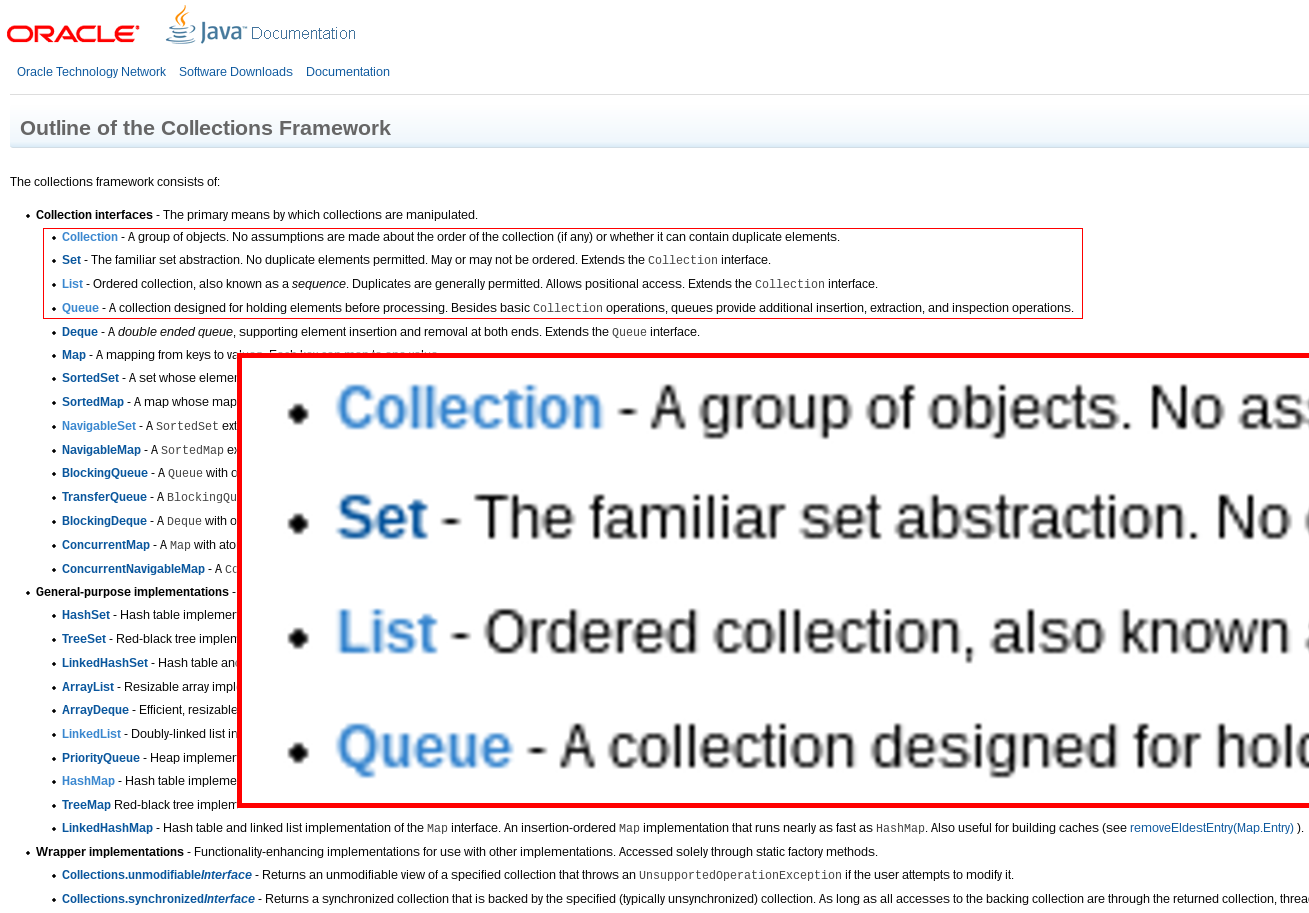
\includegraphics[scale=.28]{img/javacollectionsframework.png}
    \end{figure}
\end{frame}

\begin{frame}{Read the fine manual}
    \Large{\url{https://docs.oracle.com/javase/8/docs/api}}
\end{frame}



\section{Testen}

\begin{frame}{Testen}
    \textsc{\LARGE{Murphy's law}}\\
    \textsc{Anything that can go wrong will go wrong.}
\end{frame}

\begin{frame}{Testen}
    \textsc{\LARGE{Corollary}}\\
    \textsc{If there is a possibility of several things going wrong, the one that will cause the most damage will be the one to go wrong.}
\end{frame}

\begin{frame}{Testen}
    \textit{Was habe ich überhaupt davon ?}
    \begin{itemize}
        \item Testen ermöglicht es, Software-Fehler zu finden um diese dann zu korrigieren !
        \item Dabei versucht man möglichst viele verschiedene Situationen abzudecken, in denen etwas schieflaufen kann.
        \begin{itemize}
            \item e.g., viele unterschiedliche Benutzereingaben\dots
        \end{itemize}
    \end{itemize}
\end{frame}

\begin{frame}{Testen}
    \textit{Wann habe ich mein Programm genug getestet ?}
    \pause
    \begin{itemize}
        \item Nie.
        \pause
        \item Die sinnvollere Frage lautet: \quotes{\textbf{Wie sehen gute Testfälle aus ?}}
    \end{itemize}
\end{frame}

\begin{frame}{Testen}
    \textit{Wie sehen gute Testfälle aus ?}
    \pause
    \begin{itemize}
        \item Typische Vorgehensweise:
        \begin{enumerate}
            \item Klassifizierung der möglichen Eingabedaten (Standardsituationen und Randfälle betrachten)
            \item Auswahl der repräsentativen Daten zu jedem Testfall
        \end{enumerate}

        \item Prüfen genau eine spezifische Eigenschaft ab.
        \item Kurz und knapp.
        \item Können isoliert ausgeführt werden.
        \item Orientieren sich an der Spezifikation (i.e., Aufgabenstellung)
    \end{itemize}
\end{frame}


\begin{frame}{Testen}
    \Large{\quotes{Testing shows the presence, not the absence of bugs.}}\\
    \vspace{.4in}
    \textit{- Dijkstra}
\end{frame}



\begin{frame}{Fragen ?}
    \begin{figure}
        
\includegraphics[scale=.5]{img/question_to_idea.jpg}
    \end{figure}
\end{frame}

\appendix
\beginbackup

\begin{frame}{Bis nächste Woche !}
    \begin{figure}
        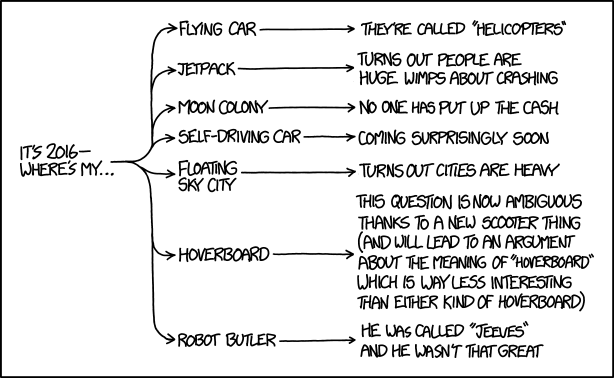
\includegraphics[scale=.5]{img/2016.png}
    \end{figure}

    \begin{flushright}
    \footnotesize{xkcd.com}
    \end{flushright}
\end{frame}

\backupend

\end{document}
